% C.20 □ABCD, ∠A=70°
\documentclass[tikz,border=4pt]{standalone}
\usepackage{ctex}
\usepackage{amsmath}
\usetikzlibrary{calc, arrows.meta}
\begin{document}
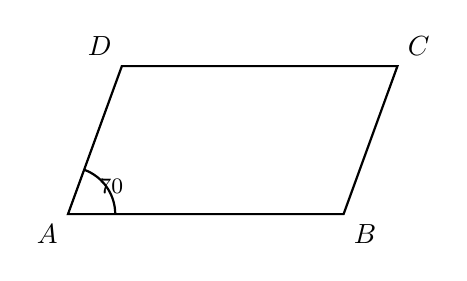
\begin{tikzpicture}[scale=1.0, thick]
  \coordinate (A) at (0,0);
  \coordinate (B) at (3.5,0);
  \coordinate (D) at ({2*cos(70)},{2*sin(70)});
  \coordinate (C) at ($(B)+(D)$);
  \draw (A) -- (B) -- (C) -- (D) -- cycle;
  \node[below left] at (A) {$A$};
  \node[below right] at (B) {$B$};
  \node[above right] at (C) {$C$};
  \node[above left] at (D) {$D$};
  \draw (0.6,0) arc (0:70:0.6);
  \node[font=\footnotesize] at (0.55,0.35) {$70°$};
\end{tikzpicture}
\end{document}
